%
% teil3.tex -- Beispiel-File für Teil 3
%
% (c) 2020 Prof Dr Andreas Müller, Hochschule Rapperswil
%
% !TEX root = ../../buch.tex
% !TEX encoding = UTF-8
%


\section{Harmonische Systeme und Rauschen\label{brown:Rauschen}}
\rhead{Implikationen}

Um dem Thema des Buches gerecht zu werden und dieses Kapitel einzugliedern, kann die harmonische Analysis als essenzielles Werkzeug betrachtet werden, um mit Rauschen umzugehen und dieses zu charakterisieren. 
So ist zum Beispiel die \textit{Fast Fourrier Transform} eine wichtige Methode, um periodische Signale von Rauschen unterscheiden zu können. 
Weiter können mittels harmonischer Analysis auch Filter entwickelt werden, welche ein Signal von Rauschen befreien. Ein gutes Beispiel dafür sind Bandpassfilter, welche nur ein bestimmtes Band an Frequenzen durchlassen.


Für viele Anwendungen ist es auch möglich mittels hochfrequenter überlagerten Schwingungen Rauschen zu modellieren. Dies ist natürlich nur eine Annäherung, da "echtes" Rauschen - je nach Fachbereich und Definition - weder vorhersagbar sein sollte, noch Information beinhaltet. 
Durch die Analyse von Systemantworten auf verschiedene harmonische Anregungen kann eine Aussage getroffen werden, wie das System auf Rauschen - also eine zufällige Störung - reagieren könnte.


All diese Beispiele basieren auf Methoden der Harmonischen Analysis. Um den Bogen zur Anfangsbemerkung dieses Kapitels zu schliessen: Durch Zufälle kann Rauschen entstehen, was meist ungewollt ist. Rauschen kann als "Gegenteil" der harmonischen Analysis erachtet werden, obwohl dafür keine klare mathematische Definition besteht. Dank Methoden der hamronsichen Analysis ist es möglich diese gegenteiligen Eigenschaften zu untersuchen und zu bewerten.


\subsection{Was ist Rauschen?\label{brown:Rauschen:Arten}}
Rauschen ist in vielen technischen und wissenschaftlichen Disziplinen ein wichtiger Faktor. So kann es auch in verschiedenen Kontexten unterschiedlich definiert werden. Zum Beispiel in der Signal- und Kommunikationstechnik kann Rauschen als zufällige ungewollte Störung beschrieben werden. 


Mathematisch können unterschiedliche Arten von Rauschen beschrieben werden, einige der wichtigsten sind folgende: 
% https://www.elektroniktutor.de/elektrophysik/rauschen.html

\begin{definition}{\bf Weisses Rauschen:}
	\begin{itemize}
		\item Alle Frequenzen haben die gleiche Amplitude.
		\item Das Leistungsdichtespektrum ist konstant über alle Frequenzen. 
	\end{itemize}
Ein Beispiel dafür ist das Rauschen von Radios, wenn die Frequenz nicht ganz eingestellt ist. Zu diesen Störeinflüsse zählen zum Beispiel: Elektrische Interferenzen, kosmische Einflüsse oder auch Blitzentladungen. Analog zu weissem Licht, kann weisses Rauschen so interpretiert werden, dass sich verschiedene Frequenzen überlagern, wobei anzumerken ist, dass weisses Licht kein konstantes Frequenz-Spektrum aufweisst.
\end{definition}

\begin{definition}{\bf Rosa Rauschen}
	\begin{itemize}
		\item Die Amplitude des Rauschens nimmt mit zunehmender Frequenz ab, ist also invers proportional zur Frequenz ($ 1/f $).
		\item Ist technisch in der Elektronik relevant und mit 3 dB Abfall der Leistungsdicht pro Oktave charakterisiert.
	\end{itemize}
Um bei einem hörbaren Beispiel zu bleiben: Rosa Rauschen klingt als Schall ausgewogener und "weicher" als weißes Rauschen. Dies, da unangenehme hohe Frequenzen wegfallen. Der Begriff "Rosa" ist eine Analogie zum sichtbaren Licht, bei dem tiefere Frequenzen auch eher rötlich erscheinen und überlagert mit Weiss (weisses Rauschen), Rosa ergeben.
\end{definition}

\begin{definition}{\bf Braunes Rauschen (Brownschess Rauschen):}
	\begin{itemize}
		\item Die Amplituden des Rauschens nehmen mit zunehmender Frequenz invers quadratisch ab ($ 1/f^2 $).
		\item Ist auch technisch relevant und mit 6 dB Abfall der Leistungsdicht pro Oktave charakterisiert.
	\end{itemize}
"Braun" bezieht sich hier nicht auf eine Farbe, sondern ist Robert Brown gewidmet. Denn die Brownische Modekühlbewegung entspricht diesem Rausch-Typ, da sich die beobachteten trägen Moleküle mit zunehmender Frequenz verstärkt gegenseitig behindern.
\end{definition}

\begin{definition}{\bf Gaussisches Rauschen:}
	\begin{itemize}
		\item Die Leistungsdichte weist bezüglich der Amplituden eine Normalverteilung (Gauß-Verteilung) um eine zentrale Frequenz auf.
	\end{itemize}
Diese Art von Rauschen ist auf digitalen Bildern zu finden deshalb speziell für die digitale Bildverarbeitung relevant. 
\end{definition}

\begin{definition}{\bf Impulsrauschen:}
	\begin{itemize}
		\item Plötzliche, unerwartete Spitzen der Amplitude 
		\item Nicht kontinuierlicher Signalverlauf (skalierter Impuls)
		\item Eine unregelmässig verteilte Leistungsdichte
	\end{itemize}
In der Bildverarbeitung ist diese Art von Rauschen als \textit{slat \& pepper Rauschen} bekannt, bei dem einzelne Pixel plötzlich extreme Werte annehmen. Dies wirkt visuell auf dem Bild wie verstreutes Salz oder Pfeffer.
\end{definition}

Es gibt noch viele weitere Unterscheidungen, doch auf diese wird nicht eingegangen. Man merkt, dass sich eine Verbindung zur harmonischen Analysis knüpfen lässt. Rauschen wird vielfach neben der Intensität bezüglich des Frequenzbereichs und der Verteilung der Amplituden charakterisiert.


% Absatz?
Es gibt aber auch Signale, welche wie Rauschen wirken können, jedoch kein Rauschen sind. So zum Beispiel hochfrequente überlagerte Schwingungen. Diese Überlagerungen sind in der Nachrichtentechnik häufig anzutreffen als auf modulierte Signale oder auch überlagerte Signale verschiedener Frequenzen um mehr Information über den selben Signalträger zu senden.
 
 
In den zwei Abbildungen ~\ref{stochastischesRauschen} \& ~\ref{überlagerteSchwingungen} sind zwei Signale aufgetragen - eines stellt echtes stochastisches Rauschen dar, das andere besteht aus vielen hochfrequenten überlagerten Schwingungen. Dieses Beispiel soll verdeutlichen, dass es nicht reicht nur den zeitlichen Verlauf eines Signals zu betrachten. So könnte man fälschlicherweise die Signale als ähnlich erachten - eine krasse Täuschung, welche sich im Frequenzspektrum klar zeigt - um das Signal zu verstehen, sind also die Methoden  der harmonischen Analysis essenziell. 

\begin{figure}
	\centering
	\begin{minipage}{0.45\textwidth}
		\centering
		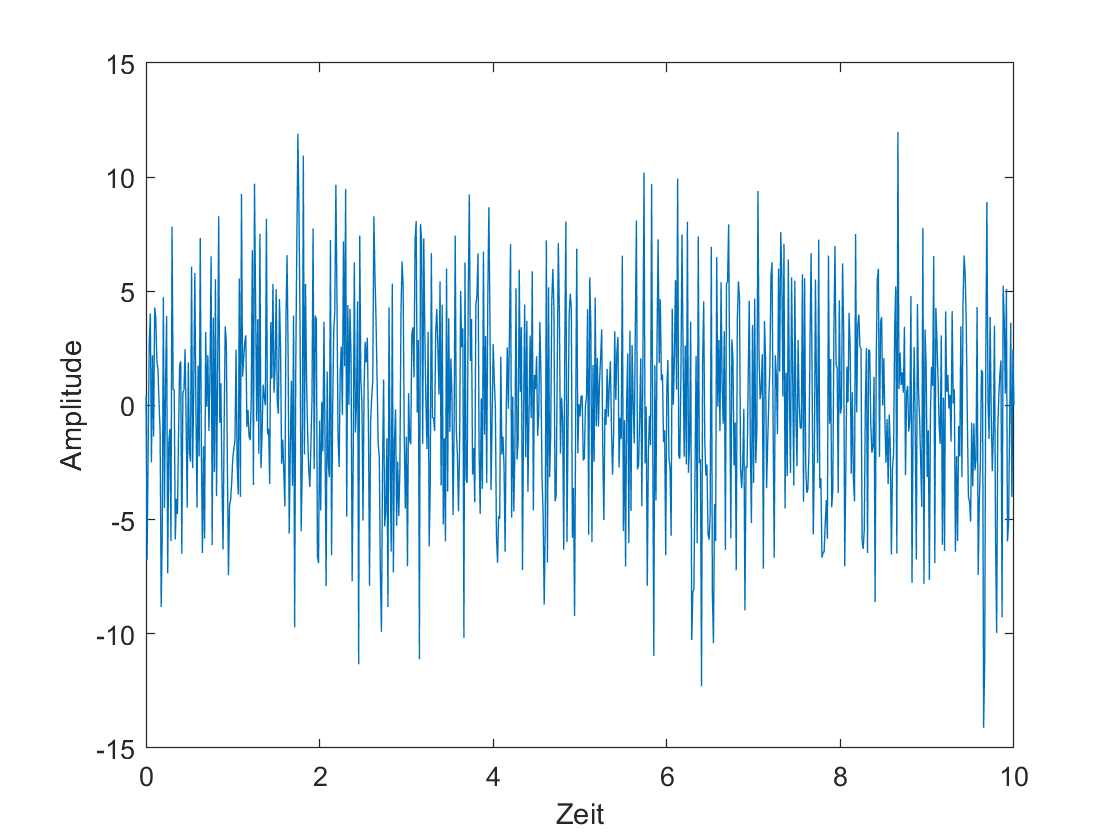
\includegraphics[width=\linewidth]{papers/brown/images/weissesRauschen.png}
		\caption{Echtes weisses Rauschen}
		\label{weissesRauschenSignal}
	\end{minipage}
	\hspace{0.05\linewidth}
	\begin{minipage}{0.45\textwidth}
		\centering
		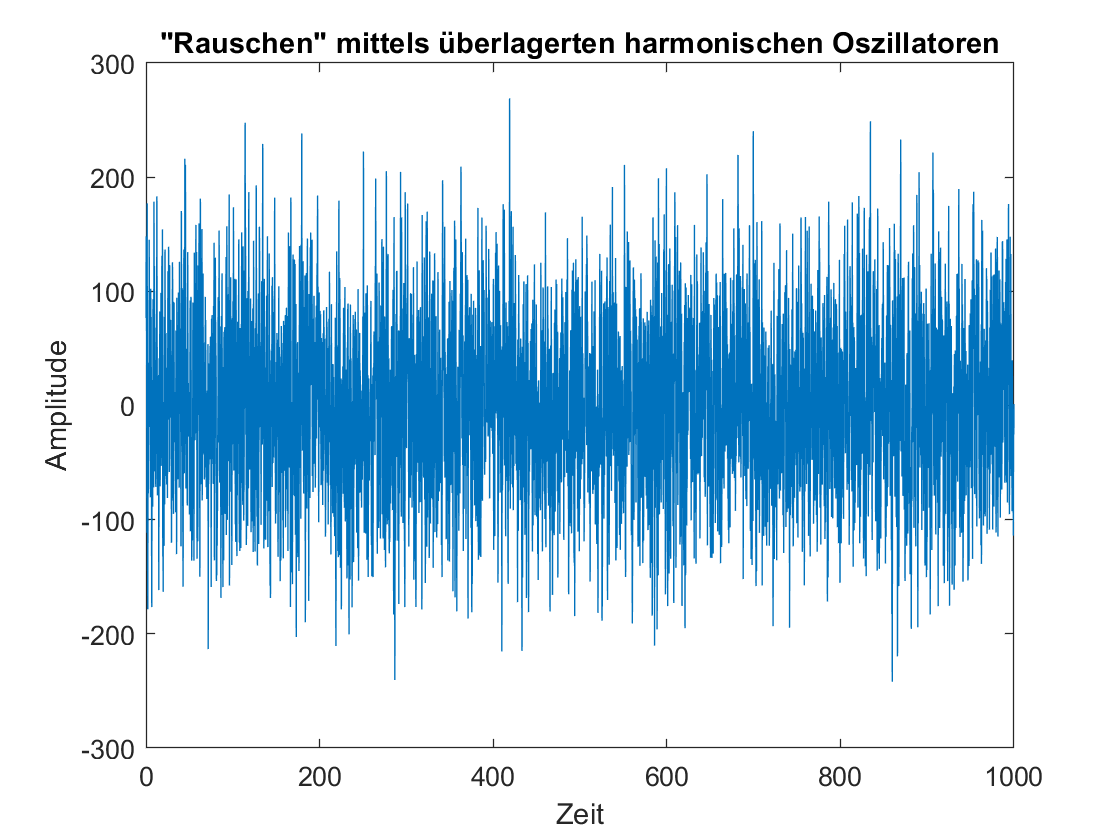
\includegraphics[width=\linewidth]{papers/brown/images/RauschenDurchUeberlagerteHarmonsicheSchwingungen.png}
		\caption{Überlagerte harmonische Schwingungen}
		\label{überlagerteSchwingungen}
	\end{minipage}
		\begin{minipage}{0.45\textwidth}
		\centering
		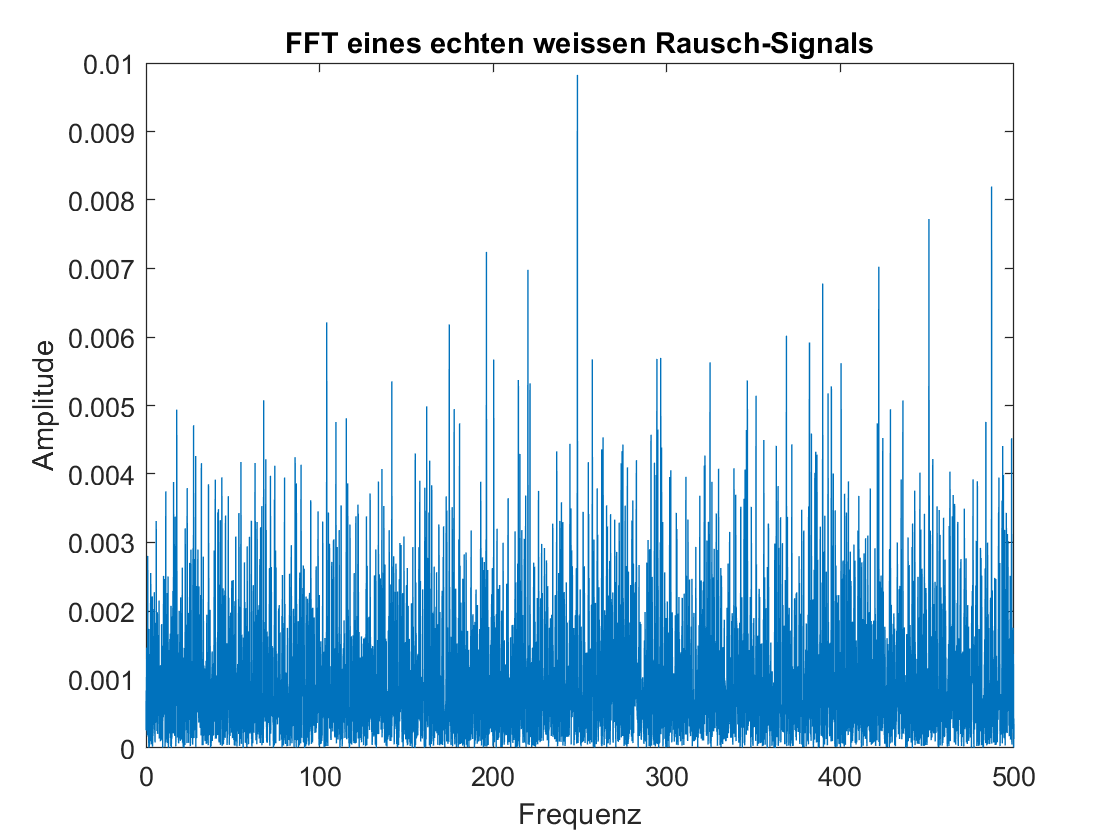
\includegraphics[width=\linewidth]{papers/brown/images/FFTweissesRauschen.png}
		\caption{FFT eines weissen Rausch-Signals}
		\label{FFTweissesRauschen}
	\end{minipage}
	\hspace{0.05\linewidth}
	\begin{minipage}{0.45\textwidth}
		\centering
		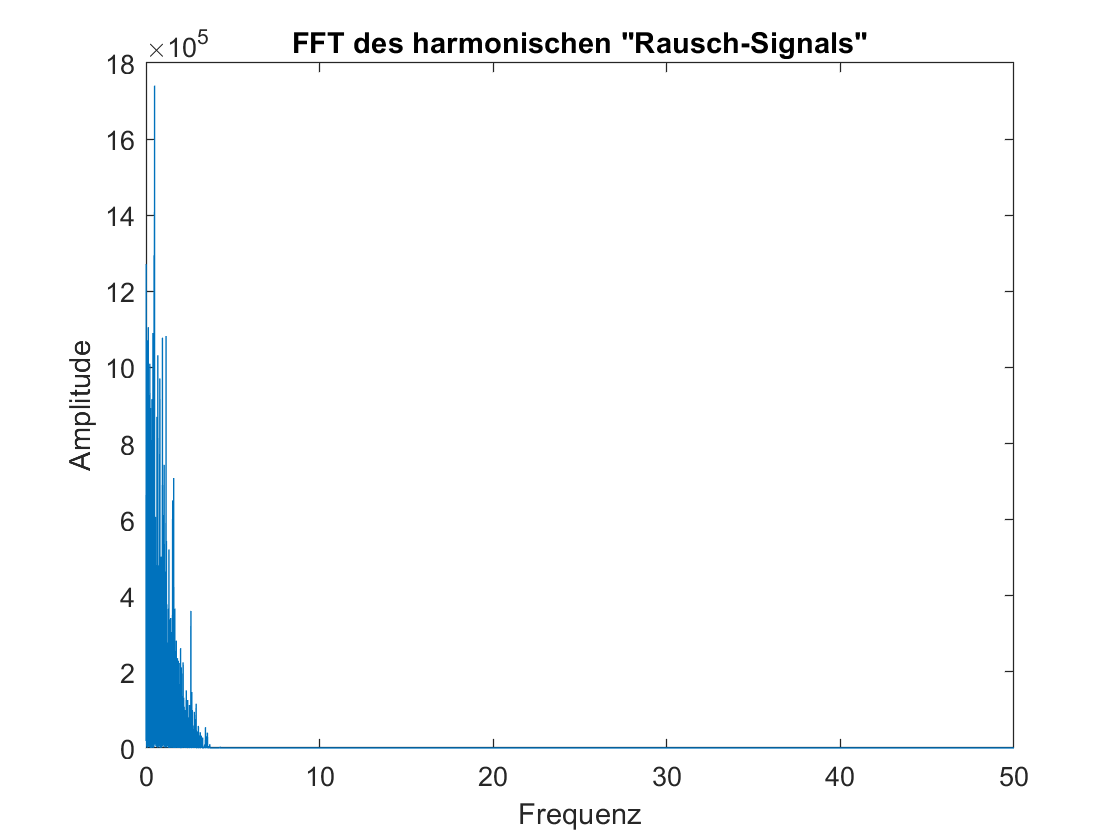
\includegraphics[width=\linewidth]{papers/brown/images/FFT-ueberlagerteSchwingungen.png}
		\caption{FFT von überlagerten harmonischen Schwingungen}
		\label{FFTüberlagerteSchwingungen}
	\end{minipage}
\end{figure}


\subsection{Rauschen mittels Random Walk oder Wiener Prozess\label{brown:Rauschen:RandomWalkWiener}}

Um Rauschen zu modellieren muss als Grundlage ein stochastischer Prozess definiert werden. Zwei zentrale Konzepte sind dabei der \textit{random walk} und der Wienerprozess.

\begin{definition}\textbf{Random Walk:}
	\label{randomWalk}
	Bei einem Random Walk beginnt man an einem Ausgangspunkt (normalerweise 0) und macht bei jedem Zeitschritt eine zufällige Schritt nach vorne oder hinten, oft dient dazu die Binominalverteilung, wobei auch asymmetrische Verteilungen verwendet werden können. Die Schrittlänge und Richtung kann ebenfalls durch eine unabhängige Wahrscheinlichkeitsverteilung bestimmt werden order als konstant definiert sein.
\end{definition}

\begin{definition}\textbf{Wiener-Prozess:}
	\label{wienerprozess}
	Der Wiener-Prozess ist ein kontinuierlicher stochastischer Prozess, er kann als Grenzwert eines Random Walks betrachtet werden, wenn die Zeitschritte gegen null gehen und die Schrittlängen normalverteilt sind. Speziell dabei ist, dass unabhängig von der verstrichenen Zeit der Erwartungswert dem Ausgangswert entspricht.	
\end{definition}

Er muss also folgende Eigenschaften erfüllen: 

%Man könnte also den Random Walk als eine diskrete Version eines Wiener-Prozesses bezeichnen oder umgekehrt, dass ein Wiener-Prozess eine kontinuierliche Version eines Random Walks ist. Sie unterscheiden sich jedoch bezüglich ihrer zeitlichen Diskretisierung und in den verwendeten Wahrscheinlichkeitsverteilungen.


\begin{enumerate}
	\item $ W(0) = 0 $; Der Startwert von $ t = 0 $ ist 0.
	\item $ W(t_{1}) - W(t_{2}) $ ist ein normalverteilte Zufalls-Variable mit Erwartungswert 0 und Varianz $ t_{1} - t_{2} $.
	\item Zu jedem weiteren Zeitpunkt $ t_{n} $ ist die Zufalls-Variable unabhängig von allen vorhergehenden Werten. Dies wird auch die Markow-Eigenschaft genannt, wenn der Übergang in einen neuen Zustand nicht vom vorherigen verlauf abhängt.
\end{enumerate}

Weiter wird auf den Wienerprozess jedoch nicht eingegangen, da dieser ausführlich im Kapitel \glqq \textit{8.1 Modell für Rauschen: der Wiener-Prozess}\glqq{} des Buches vom Mathematischen Seminar über Differenzialgleichungen beschrieben wird. ???Abstand???


\subsection{Implikationen\label{brown:Rauschen:Implikationen}}

- Differnezierbarkeit
\begin{figure}
	\centering
	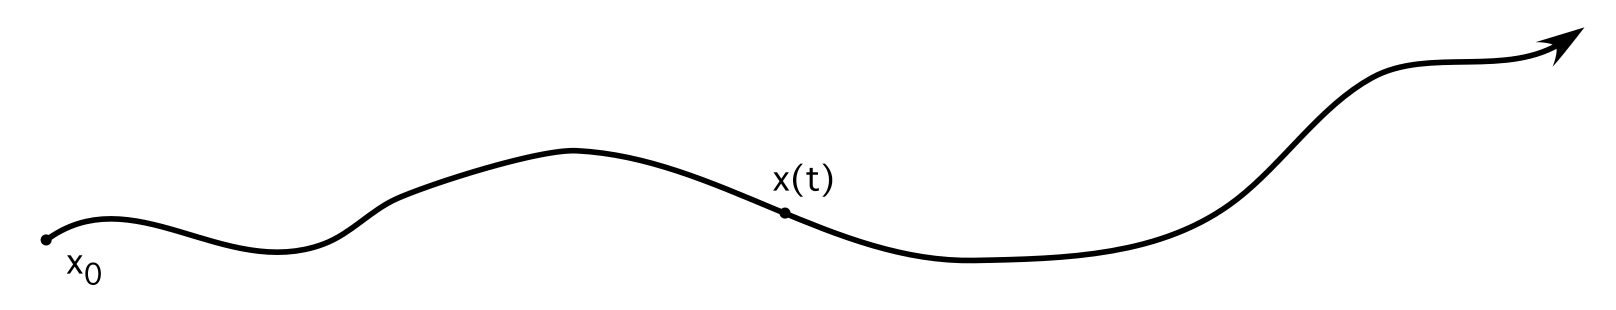
\includegraphics[width=0.3\textwidth]{papers/brown/images/idealSignal.png}
	\caption{Ideales Signal}
	\label{idealSignal}
\end{figure}
\begin{figure}
	\centering
	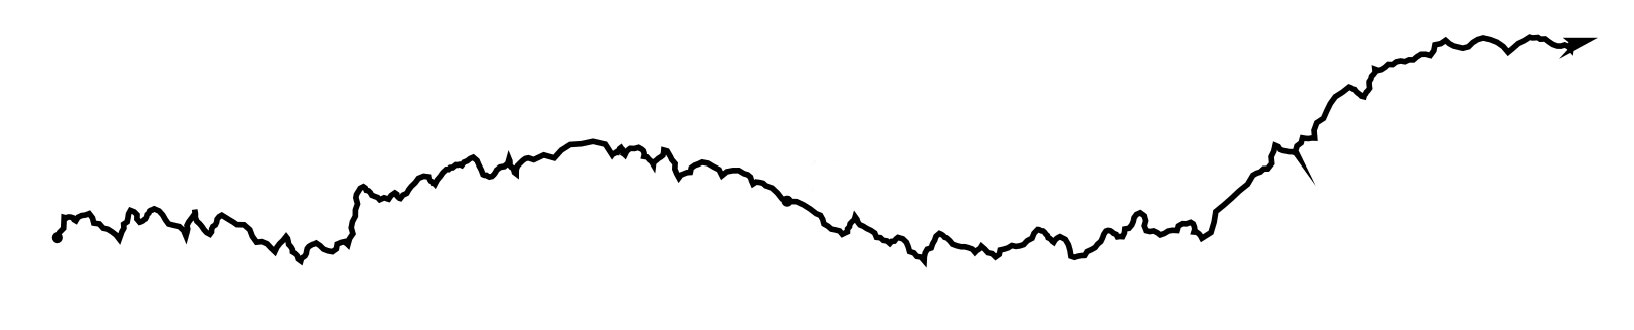
\includegraphics[width=0.3\textwidth]{papers/brown/images/realSignal.png}
	\caption{Reales Signal}
	\label{realSignal}
\end{figure}

Ohne Methoden der stoachstischen Differenzialrechnung kann kaum ein SIgnal anhand von verrauschten Daten oder von zufällig gestörten Systemen erstellt werden. In der Sign


- Gefahr von Instabilität